\documentclass[a4paper]{article}
\usepackage[utf8]{inputenc}
\usepackage{textcomp}
\usepackage{geometry}
\geometry{ left=2cm, right=2cm, top=2cm, bottom=2cm, bindingoffset=5mm}
\usepackage{graphicx}
\usepackage{xcolor}
\usepackage{hyperref}
\date{}
\author{}
\usepackage{fancyhdr}
\pagestyle{fancy}
\fancyhf{}
\fancyhead[R]{Felix Bühler - 2973140\\ Jan Leusmann - 2893121\\  Jamie Ullerich - 3141241}
\fancyhead[L]{Reinforcement Learning \\ SS 2020}
\renewcommand{\headrulewidth}{0.5pt}
\usepackage{tikz}
\usetikzlibrary{calc}
\usepackage{amsmath}
\usepackage{cleveref}
\usepackage{subcaption}
\usepackage{array}
\usepackage{bbold}
\usepackage{listings}

\title{\textbf{Exercise 6}}

\begin{document}
\maketitle 
\thispagestyle{fancy}

\section*{Task 1 - Planning and Learning}

\begin{enumerate}
	\item[a)] In Dyna-Q, in every step all Q(s,a) are updated, which leads to a better performance.
	\item[b)] The cumulative reward for the Dyna-Q+ agent is higher since he will get a special bonus reward for testing all accessible state transaction (especially those who have not been considered in a long time). 
\end{enumerate}

\section*{Task 2 - n-step sarsa on the FrozenLake}
\begin{figure}[!ht]
	\centering
	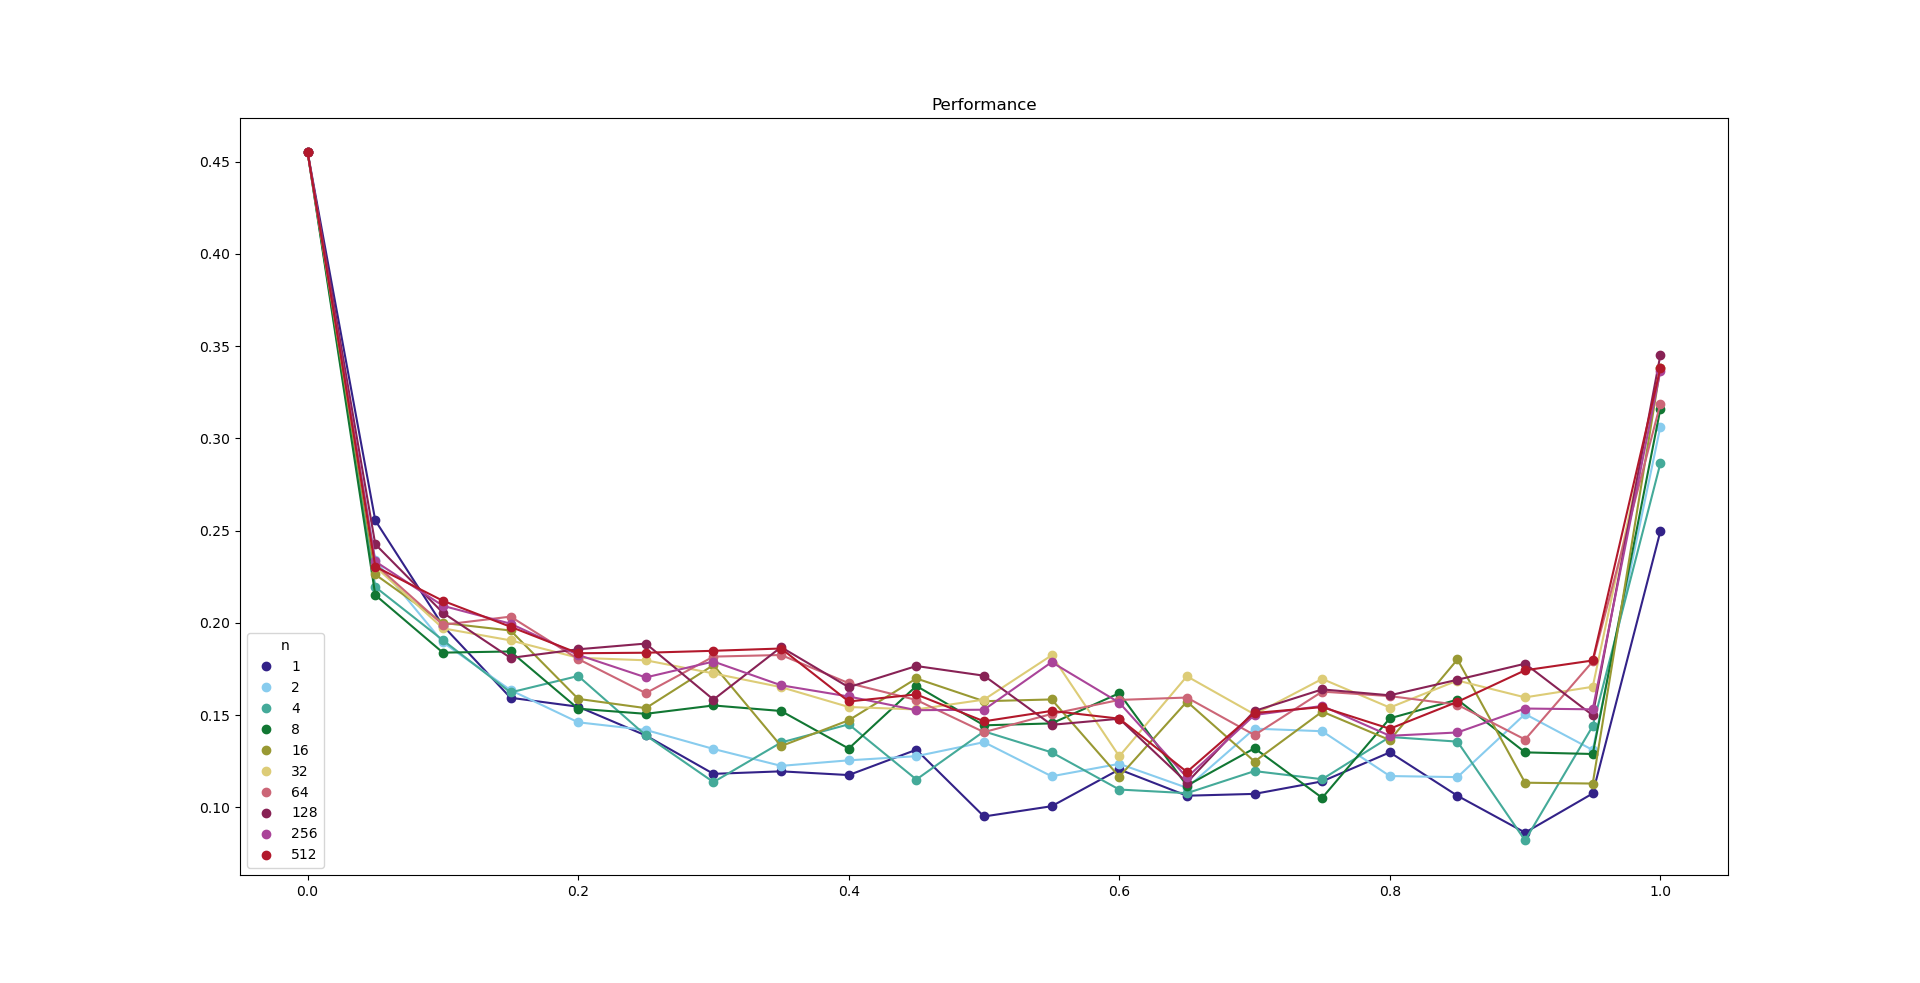
\includegraphics[width=0.7\linewidth]{ex6_2}
	\caption{y-axis: RMS of Q\_values, x-axis: alpha values}
	\label{fig:ex62}
\end{figure}


\end{document}
